\documentclass{standalone}
\usepackage{tikz}
\usetikzlibrary{fit}

\begin{document}
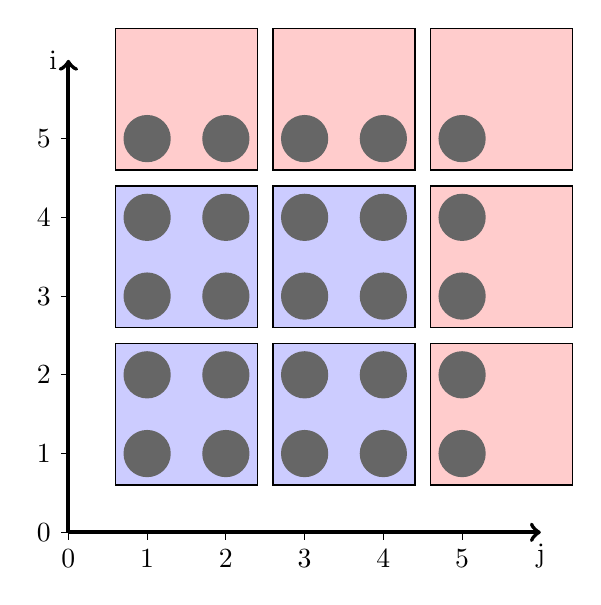
\begin{tikzpicture}
\tikzset{axis/.style={draw=black,->,line width=1.5pt}}
\tikzset{reddot/.style={fill=red,circle,inner xsep=0mm,inner ysep=0mm,minimum width=6mm,anchor=center}}
\tikzset{bluedot/.style={fill=blue,circle,inner xsep=0mm,inner ysep=0mm,minimum width=6mm,anchor=center}}
\tikzset{dot/.style={fill=black!60,circle,inner xsep=0mm,inner ysep=0mm,minimum width=6mm,anchor=center}}
\tikzset{completetile/.style={draw=black,->,line width=0.5pt,fill=blue!20}}
\tikzset{partialtile/.style={draw=black,->,line width=0.5pt,fill=red!20}}



\path[axis] (0,0) -- (6,0) node[below](i)  {j};
\foreach \x in {0,...,5} {
  \path[draw] (\x,0) -- ++(0,-0.1) node[below] {\x};
}

\path[axis] (0,0) -- (0,6) node[left](j) {i};
\foreach \y in {0,...,5} {%
  \path[draw] (0,\y) -- ++(-0.1,0) node[left]() {\y};%
}

\node[use as bounding box,fit={(0,0) (6,6)}]{};


\path[completetile] ([xshift=-0.4cm,yshift=-0.4cm]1,1) rectangle ([xshift=0.4cm,yshift=0.4cm]2,2);
\path[completetile] ([xshift=-0.4cm,yshift=-0.4cm]3,1) rectangle ([xshift=0.4cm,yshift=0.4cm]4,2);
\path[completetile] ([xshift=-0.4cm,yshift=-0.4cm]1,3) rectangle ([xshift=0.4cm,yshift=0.4cm]2,4);
\path[completetile] ([xshift=-0.4cm,yshift=-0.4cm]3,3) rectangle ([xshift=0.4cm,yshift=0.4cm]4,4);

\path[partialtile] ([xshift=-0.4cm,yshift=-0.4cm]5,5) rectangle ([xshift=0.4cm,yshift=0.4cm]6,6);
\path[partialtile] ([xshift=-0.4cm,yshift=-0.4cm]1,5) rectangle ([xshift=0.4cm,yshift=0.4cm]2,6);
\path[partialtile] ([xshift=-0.4cm,yshift=-0.4cm]3,5) rectangle ([xshift=0.4cm,yshift=0.4cm]4,6);
\path[partialtile] ([xshift=-0.4cm,yshift=-0.4cm]5,1) rectangle ([xshift=0.4cm,yshift=0.4cm]6,2);
\path[partialtile] ([xshift=-0.4cm,yshift=-0.4cm]5,3) rectangle ([xshift=0.4cm,yshift=0.4cm]6,4);


\foreach \x in {1,...,5} {
    \foreach \y in {1,...,5} {
        \node[dot] at (\x,\y) {};
    }
}
\end{tikzpicture}
\end{document}
